\chapter{Revisão de literatura e fundamentos da stack tecnológica}
\label{cap:revisao}
% --------------------------------------------------------------------------

\section{O ecossistema de nanossatélites e a engenharia de sistemas nacional}
\label{sec:ecossistema}

A consolidação da arquitetura \textit{CubeSat}, estabelecida no final da década de 1990 pelo padrão \textit{CubeSat Design Specification} (CDS) formulado pela California Polytechnic State University e pela Stanford University (CALIFORNIA POLYTECHNIC STATE UNIVERSITY, 2022), promoveu uma mudança de paradigma na exploração espacial. Ao padronizar as dimensões geométricas em múltiplos inteiros de uma unidade cúbica fundamental (1U) com aresta nominal de \SI{100.0}{\milli\metre} e massa unitária de até \SI{1.33}{\kilo\gram}, a norma substituiu o desenvolvimento customizado e artesanal por uma plataforma aberta e modular. Essa padronização viabilizou o emprego sistemático de componentes comerciais de prateleira (\textit{Commercial Off-The-Shelf} -- COTS), reduzindo em ordens de magnitude o custo de fabricação e o tempo de desenvolvimento de missões orbitais.

No cenário aeroespacial brasileiro, a Agência Espacial Brasileira (AEB), em cooperação com o Instituto Nacional de Pesquisas Espaciais (INPE) e o Instituto Tecnológico de Aeronáutica (ITA), estruturou diretrizes formais para o ciclo de vida e a certificação de pequenas plataformas satelitais. Conforme sistematizado na \textit{Apostila da Temática -- Projeto Estrutural de Nanossatélites} (AEB, 2026), o chassi estrutural atua como a espinha dorsal da plataforma espacial, sendo responsável por:
\begin{enumerate}
  \item suportar os esforços inerciais e dinâmicos gerados durante a queima dos estágios do foguete;
  \item manter o alinhamento óptico, mecânico e magnético de cargas úteis e sensores de controle de atitude;
  \item prover caminhos térmicos para a dissipação de calor gerado pela eletrônica de potência;
  \item atenuar os choques mecânicos decorrentes das operações de separação e ejeção orbital em órbita baixa terrestre (\textit{Low Earth Orbit} -- LEO).
\end{enumerate}

O desenvolvimento do nanossatélite universitário brasileiro ITASAT-1 (CARRARA \textit{et al.}, 2017), lançado em 2018, e a missão conjunta SPORT (\textit{Scintillation Prediction Observations Research Task}) (SANTOS \textit{et al.}, 2020) demonstraram que as campanhas de Montagem, Integração e Testes (AIT), realizadas no Laboratório de Integração e Testes (LIT/INPE), constituem a etapa mais crítica do desenvolvimento. Levantamentos empíricos globais de confiabilidade de nanossatélites — como a base histórica de dados de falhas mantida por Swartwout (2023) — revelam que aproximadamente \SI{40}{\percent} dos nanossatélites lançados sofrem anomalias funcionais severas ou perda total de missão nos primeiros 30 dias após o lançamento. Análises forenses demonstram que uma fração substancial dessas anomalias decorre de danos mecânicos cumulativos induzidos por vibração aleatória e choque de separação: trincas por fadiga em juntas soldadas de circuitos integrados, fadiga em conectores de barramento PC/104, afrouxamento de fixadores roscados e deformações residuais que provocam o travamento cinemático do satélite no interior do lançador (SLEJKO \textit{et al.}, 2023).

\section{Ambiente dinâmico de lançamento e mecânica do dispensador orbital P-POD}
\label{sec:dinamica-ejecao}

\subsection{Espectros de aceleração e requisitos normativos da NASA GEVS}
\label{subsec:gevs-norma}

O envelope dinâmico imposto a uma carga secundária durante o voo propulsado divide-se em três regimes físicos simultâneos:
\begin{alineas}
  \item \textbf{acelerações quase estáticas:} cargas sustentadas de manobra e empuxo contínuo dos motores (\SIrange{10}{20}{\gacc});
  \item \textbf{vibração acústica e turbulenta aleatória:} excitação estocástica de banda larga (\SIrange{20}{2000}{\hertz}) transmitida através da coifa do lançador;
  \item \textbf{choques mecânicos transitórios:} pulsos impulsivos de alta intensidade causados pela atuação de atuadores pirotécnicos e pela liberação de molas de ejeção.
\end{alineas}

Para garantir que o nanossatélite não sofra falha estrutural nem comprometa o veículo lançador, a certificação espacial é governada pela norma internacional \textit{General Environmental Verification Standard} (GEVS) (NASA, 2013), consubstanciada no documento NASA GSFC-STD-7000A. A norma estabelece que a estrutura primária deve ser qualificada sob um perfil de Densidade Espectral de Potência (PSD) de vibração aleatória com nível global eficaz de
\begin{equation}
  \Grmsbase = \SI{14.1}{\Grms}
  \label{eq:gevs-grms-teoria}
\end{equation}
aplicado sequencialmente nos três eixos ortogonais ($X, Y, Z$) durante \SI{120.0}{\second} por eixo. Em paralelo, a norma exige que a primeira frequência própria fundamental do satélite satisfaça:
\begin{equation}
  f_1 \ge \SI{100.0}{\hertz}
  \label{eq:f1-teoria}
\end{equation}
assegurando desacoplamento dinâmico perante os modos fundamentais de flexão e oscilações axiais do foguete (MALAVOLTA; MORENO, 2026).

\subsection{Cinemática de ejeção no P-POD e restrições tribológicas de contato}
\label{subsec:ppod-mecanica}

A interface de confinamento mecânico mais difundida na indústria aeroespacial para CubeSats é o dispensador \textit{Poly-Picosatellite Orbital Deployer} (P-POD), desenvolvido pela California Polytechnic State University (PUIG-SUARI; TURNER; AHLGREN, 2002), esquematizado na Figura~\ref{fig:ppod}.

\begin{figure}[htb]
  \caption{Diagrama explodido e interfaces mecânicas do dispensador orbital P-POD}
  \label{fig:ppod}
  \begin{center}
    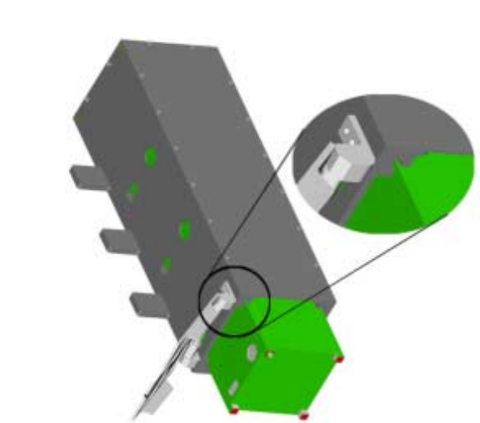
\includegraphics[width=0.7\textwidth]{figuras/ppod_explodido.png}
  \end{center}
  \fonte{Adaptado de Puig-Suari, Turner e Ahlgren (2002).}
\end{figure}

O mecanismo do P-POD fundamenta-se no confinamento do satélite no interior de uma canaleta retangular de alumínio, apoiado sobre uma placa empurradora acoplada a uma mola helicoidal comprimida. A dinâmica de ejeção translacional do satélite é descrita pela equação de movimento expressa na Equação~\eqref{eq:ejecao_teoria} (LIMA; MANEA; SANTOS, 2021):
\begin{equation}
  M\,\ddot{z}(t) + \mu N \operatorname{sgn}(\dot{z}(t)) = P_0 - c\,z(t)
  \label{eq:ejecao_teoria}
\end{equation}
onde $M$ denota a massa combinada do nanossatélite e da placa empurradora, $\ddot{z}$ representa a aceleração translacional instantânea, $P_0$ é a pré-carga inicial da mola comprimida, $c$ é a rigidez elástica da mola, $\mu$ representa o coeficiente de atrito cinemático contra as guias do tubo, $N$ é a força normal de contato gerada por desalinhamentos e folgas, e $z$ é a coordenada axial percorrida ao longo do curso total ($z \in [0, z_{\text{curso}}]$).

Sob a perspectiva da engenharia mecânica de precisão e da tribologia espacial, o confinamento no P-POD impõe que os quatro vértices longitudinais do nanossatélite atuem como patins de deslizamento direto em contato metal-metal contra as paredes internas do tubo lançador. As especificações da CDS Rev. 14 (CALIFORNIA POLYTECHNIC STATE UNIVERSITY, 2022) estipulam restrições construtivas rígidas:
\begin{alineas}
  \item os quatro trilhos devem ser monolíticos e contínuos ao longo de todo o comprimento de \SI{113.5}{\milli\metre}, com seção transversal maciça de no mínimo \rail{} e cantos arredondados com raio $R \ge \SI{1.0}{\milli\metre}$;
  \item a rugosidade superficial das faces de contato deve obedecer a $Ra \le \SI{1.6}{\micro\metre}$, complementada por tratamento de anodização dura Tipo III (com impregnação de PTFE), prevenindo o travamento mecânico por atrito e mitigando o risco de microssoldagem a frio (\textit{cold welding}) das ligas de alumínio sob alto vácuo espacial;
  \item o acoplamento dimensional opera com uma folga diametral nominal (\textit{clearance}) de \SIrange{0.1}{0.3}{\milli\metre}. Essa folga impede o engastamento rígido do chassi durante o ensaio em mesa vibratória acoplada a casulo de ensaio (\textit{Test POD}), promovendo contato unilateral não linear, impactos intermitentes e vibração com folga (\textit{chattering}), os quais redistribuem os fluxos de tensão e reduzem a rigidez aparente de ressonância em relação a condições de engaste perfeito.
\end{alineas}

Consequentemente, torna-se geometricamente mandatório que os quatro trilhos longitudinais do CubeSat permaneçam sólidos e contínuos. A otimização topológica e o alívio de massa estrutural devem ser concentrados estritamente nos quatro painéis laterais internos do chassi.

\subsection{Choque de separação orbital e Espectro de Resposta ao Choque (SRS)}
\label{subsec:srs-teoria}

No término do curso axial de impulsão ($z = z_{\text{curso}}$), a placa empurradora colide abruptamente contra o batente mecânico do dispensador, transferindo um pulso transiente de desaceleração de altíssima amplitude ($\Delta t \sim \SIrange{1}{3}{\milli\second}$) que se propaga pelos trilhos do satélite no instante da separação orbital (LIMA \textit{et al.}, 2021). 

A severidade mecânica desse evento impulsivo é quantificada pelo Espectro de Resposta ao Choque (\textit{Shock Response Spectrum} -- SRS), calculado considerando uma família de osciladores de um grau de liberdade (SDOF) amortecidos com fator de qualidade canônico $\mathcal{Q} = 10$ ($\zeta = \SI{5.0}{\percent}$). Para frequências acima de \SI{1000}{\hertz}, a aceleração de pico do SRS pode ultrapassar \SI{500}{\gacc}, excitando modos ressonantes de alta frequência em placas de circuito impresso e deflagrando vibrações acopladas em apêndices articulados, tais como antenas desdobráveis, magnetômetros e painéis solares (MANTOVANI; SANTOS; CARDOSO-RIBEIRO, 2020). Essa constatação evidencia a necessidade de que os painéis celulares do chassi primário atuem como filtros passivos de ondas elásticas, atenuando a transmissão desse choque transitório para o interior do satélite.

\section{Metamateriais celulares auxéticos e propriedades mecânicas avançadas}
\label{sec:auxeticos-teoria}

\subsection{Cinemática celular e coeficiente de Poisson negativo}
\label{subsec:poisson-negativo}

Para mitigar a elevada transmissão vibratória inerente a chassis maciços contínuos sem adicionar subsistemas pesados de amortecimento, investigam-se metamateriais celulares arquitetados com coeficiente de Poisson negativo ($\nu < 0$), denominados auxéticos (LI \textit{et al.}, 2026). Na elasticidade linear isotrópica tridimensional clássica, os limites termodinâmicos da energia de deformação positiva impõem que o coeficiente de Poisson varie no intervalo restrito:
\begin{equation}
  -1.0 \le \nu \le 0.5
  \label{eq:limites-poisson}
\end{equation}
A quase totalidade dos materiais estruturais convencionais apresenta valores positivos no intervalo $0{,}25 \le \nu \le 0{,}35$. Materiais auxéticos exploram o limite inferior desse domínio termodinâmico, expandindo-se transversalmente sob tração uniaxial e contraindo-se transversalmente sob compressão.

Nas células unitárias bidimensionais e tridimensionais reentrantes (Figura~\ref{fig:falha-reentrante}), esse comportamento contra-intuitivo resulta da cinemática de rotação e flexão das costelas oblíquas com ângulo de reentrância $\theta$. Considerando o modelo cinemático de dobradiça elástica com barras de espessura $t$, comprimento oblíquo $l$, altura vertical $h$ e ângulo positivo de reentrância $\theta$ medido em relação à base horizontal celular (em que as costelas inclinam-se em direção ao interior do poro celular), o coeficiente de Poisson efetivo na flexão do plano $yx$ carrega o sinal negativo decorrente da cinemática de abertura lateral (GIBSON; ASHBY, 1997; LI \textit{et al.}, 2026):
\begin{equation}
  \nu_{yx}^* = -\frac{\sin\theta \left( \dfrac{h}{l} + \sin\theta \right)}{\cos^2\theta}
  \label{eq:poisson-analitico}
\end{equation}
Para configurações reentrantes com $\theta > 0$ (como no ponto ótimo de voo $\theta^* = \SI{65.75}{\degree}$, equivalente à deflexão angular cartesiana $\theta_{\text{def}} = -21{,}40^\circ$), a Equação~\eqref{eq:poisson-analitico} fornece um coeficiente de Poisson analítico de elevada magnitude ($\nu_{yx}^* = \num{-13.81}$, ou $\num{-12.63}$ na célula ótima discretizada), comprovando o comportamento auxético marcante da mesoestrutura celular sob flexão pura.

\paragraph{Reconciliação Multiescala do Coeficiente de Poisson}
É imperativo estabelecer a distinção entre a cinemática celular microscópica e o comportamento estrutural tridimensional macroscópico:
\begin{alineas}
  \item \textbf{escala micromecânica celular 2D isolada:} uma célula unitária desimpedida sujeita exclusivamente à flexão de suas hastes delgadas desenvolve contração lateral extrema ($\nu_{yx}^* \in [\num{-12.63}, \num{-13.81}]$) devido à mobilidade geométrica livre das arestas;
  \item \textbf{resposta estrutural contínua 3D com restrição de trilhos:} quando a rede auxética é tridimensionalizada e integrada monoliticamente aos quatro trilhos guia maciços de \rail{} e às flanges de interface em AlSi10Mg ($\nu_s = +0{,}33$), a rigidez axial dos trilhos e o confinamento cinemático das bordas atenuam a magnitude da deformação lateral global, estabelecendo um coeficiente de Poisson efetivo homogeneizado de $\nu_{\text{eff}} = \num{-0.428}$. Essa reconciliação multiescala comprova que o chassi preserva o desacoplamento dinâmico sem incorrer em instabilidades elásticas de contorno.
\end{alineas}

\begin{figure}[htb]
  \caption{Modos de falha e comportamento cinemático anisotrópico de célula reentrante 2D sob carregamento uniaxial}
  \label{fig:falha-reentrante}
  \begin{center}
    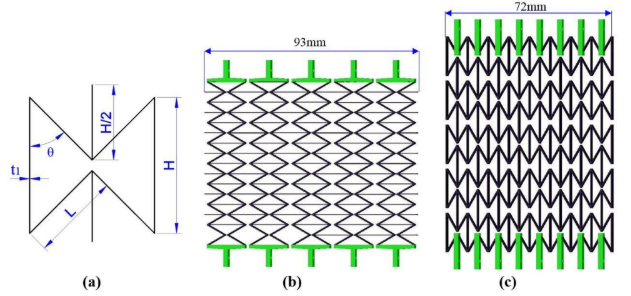
\includegraphics[width=0.85\textwidth]{figuras/modos_falha_reentrante.png}
  \end{center}
  \fonte{Adaptado de Alomarah \textit{et al.} (2017).}
\end{figure}

Essa resposta cinemática confere às treliças auxéticas propriedades mecânicas de alto valor para a engenharia aeroespacial (FARSHBAF \textit{et al.}, 2025):
\begin{alineas}
  \item \textbf{elevada Absorção Específica de Energia (\textit{Specific Energy Absorption} -- SEA):} capacidade superior de dissipar energia mecânica sob impacto e deformação plástica volumétrica confinada;
  \item \textbf{resistência mecânica à indentação e tenacidade à fratura:} sob concentração pontual de tensão, o material sofre fechamento lateral das células em direção ao ponto de carga, aumentando a densidade local e prevenindo a penetração mecânica;
  \item \textbf{deformação em curvatura sinclástica:} ao serem fletidas, placas auxéticas assumem formato de domo convexo (curvatura de mesmo sinal em ambas as direções principais), eliminando a curvatura anticlástica característica de vigas convencionais e otimizando o acoplamento com envoltórias curvas de painéis.
\end{alineas}

\subsection{Células celulares híbridas e limitações em manufatura aditiva}
\label{subsec:celulas-hibridas}

Tentativas recentes na literatura visam aumentar a rigidez e a absorção energética de células celulares através de topologias híbridas quirais-reentrantes, como proposto por Cui, Zhang e Wang (2025) (Figura~\ref{fig:hibrida-quiral}). 

\begin{figure}[htb]
  \caption{Topologia híbrida de célula celular com elementos quirais internos acoplados a paredes reentrantes}
  \label{fig:hibrida-quiral}
  \begin{center}
    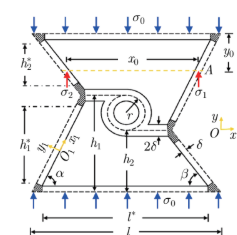
\includegraphics[width=0.55\textwidth]{figuras/celula_hibrida_quiral.png}
  \end{center}
  \fonte{Adaptado de Cui, Zhang e Wang (2025).}
\end{figure}

Embora estruturas quirais proporcionem aumentos expressivos na SEA, sua conformação tridimensional cria superfícies curvas suspensas com ângulos de inclinação inferiores ao limite crítico autossuportado da Manufatura Aditiva por Fusão em Leito de Pó a Laser ($\theta_{\text{overhang}} < \SI{35}{\degree}$). Além disso, o confinamento de cavidades curvas fechadas dificulta a purga do pó metálico não consolidado. Em contraste, a geometria reentrante tridimensional parametrizada nesta tese foi especificamente sintetizada para garantir ângulos de sobre-salha autossustentados em todas as faces oblíquas ao longo da direção vertical de deposição do laser ($\theta_{\text{overhang}} \ge \SI{35}{\degree}$), eliminando a necessidade de suportes internos sacrificiais e preservando canais desobstruídos para a evacuação de pó.

\section{Projeto para Manufatura Aditiva (DfAM) e modelos fenomenológicos de escala}
\label{sec:dfam-escala}

\subsection{O processo de Fusão em Leito de Pó a Laser (L-PBF) em AlSi10Mg}
\label{subsec:lpbf-teoria}

O processo de Manufatura Aditiva metálica por Fusão em Leito de Pó a Laser (\textit{Laser Powder Bed Fusion} -- L-PBF), governado pelo padrão internacional ISO/ASTM 52900 e 52911-1, consolidou-se como o método predominante para fabricação de componentes aeroespaciais de geometria complexa (KHAN; RICCIO, 2024). No L-PBF, uma fina camada de pó metálico atomizado a gás (espessura de camada entre \SIrange{30}{60}{\micro\metre}) é espalhada sobre uma mesa de construção por uma lâmina recobridora, e um feixe de laser de fibra de alta potência (tipicamente \SIrange{200}{400}{\watt}, diâmetro de foco de $\sim\SI{70}{\micro\metre}$) varre seletivamente as seções transversais da peça.

Durante a varredura a laser, as taxas locais de aquecimento e resfriamento superam $10^6\ \text{K/s}$, gerando uma poça de fusão microscópica altamente dinâmica que se solidifica em uma microestrutura celular ultrafina de $\alpha$-Al circundada por uma rede eutética de silício. Devido aos gradientes térmicos espaciais extremos, o componente bruto de impressão acumula elevadas tensões residuais térmicas de tração. Por essa razão, a qualificação estrutural exige obrigatoriamente a aplicação de tratamento térmico de alívio de tensões a \SI{300}{\celsius} por \SI{2.0}{\hour}, o qual promove a homogeneização microestrutural, alivia mais de \SI{80}{\percent} das tensões residuais e confere ductilidade estável ao material (SLEJKO \textit{et al.}, 2023).

\subsection{Leis clássicas e refinadas de escala de Gibson-Ashby}
\label{subsec:gibson-ashby-teoria}

Para estimar as propriedades mecânicas eficazes homogeneizadas de meios celulares sem a necessidade de discretizar cada haste em malhas refinadas de elementos finitos contínuos, utilizam-se classicamente as leis fenomenológicas de escala propostas por Gibson e Ashby (1997). A relação fundamental expressa o módulo de elasticidade efetivo macroscópico ($E^{*}$) e o limite de escoamento aparente ($\sigma_y^{*}$) em função da densidade relativa ($\rho^{*}/\rho_s$):
\begin{align}
  \frac{E^{*}}{E_s} &= C_1 \left( \frac{\rho^{*}}{\rho_s} \right)^{n} \label{eq:gibson-e} \\
  \frac{\sigma_y^{*}}{\sigma_{ys}} &= C_2 \left( \frac{\rho^{*}}{\rho_s} \right)^{m} \label{eq:gibson-sigma}
\end{align}
em que $E_s$, $\sigma_{ys}$ e $\rho_s$ correspondem, respectivamente, ao módulo de elasticidade, ao limite de escoamento e à massa específica do material metálico de base (liga AlSi10Mg), e $C_1, C_2, n, m$ são constantes topológicas. Para estruturas celulares cujo mecanismo cinemático de deformação elástica sob carregamento macroscópico é dominado pela flexão de costelas — caso típico de matrizes auxéticas reentrantes —, a teoria clássica estabelece $C_1 \approx 1{,}0$, $n \approx 2{,}0$, $C_2 \approx 0{,}3$ e $m \approx 1{,}5$ (GIBSON; ASHBY, 1997; ZHONG \textit{et al.}, 2023).

Todavia, investigações recentes apontam limitações fundamentais na formulação clássica de Gibson-Ashby quando aplicada a estruturas reticuladas fabricadas por L-PBF. Zhong \textit{et al.} (2023) demonstram que a dedução da Equação~\eqref{eq:gibson-e} repousa na hipótese de vigas delgadas de Euler-Bernoulli, válida estritamente para baixas densidades relativas ($\rho^{*}/\rho_s < \num{0.30}$) e razões de aspecto de haste $L/D > 5$. Em contrapartida, estruturas otimizadas para satélites operam frequentemente com densidades intermediárias ($\rho^{*}/\rho_s \ge \num{0.35}$), regime no qual os esforços de cisalhamento transversal e deformação axial tornam-se preponderantes. 

Além disso, Zimmerman \textit{et al.} (2026) salientam que a Equação~\eqref{eq:gibson-e} viola a continuidade no limite assintótico do material maciço contínuo ($\rho^{*}/\rho_s \to 1$), uma vez que não converge assintoticamente para o comportamento do sólido de base. Adicionalmente, defeitos característicos da fusão a laser — como rugosidade superficial em planos inclinados, microporosidades térmicas e adesão de partículas de pó semidilatadas — degradam a rigidez elástica real em relação ao modelo geométrico ideal (ZIMMERMAN \textit{et al.}, 2026).

Para corrigir essas discrepâncias físicas e reestabelecer a acurácia em meios celulares de densidade graduada, Beigrezaee, Jalali e Pugno (2026) desenvolveram uma formulação fenomenológica modificada:
\begin{equation}
  \frac{E^{*}}{E_s} = \alpha\,\beta\,C_1 \left( \frac{\rho^{*}}{\rho_s} \right)^{n}
  \label{eq:gibson-refinado-teoria}
\end{equation}
na qual $\alpha$ é o coeficiente determinístico de gradiente geométrico de espessura de parede ao longo do volume celular, e $\beta$ quantifica a perda de rigidez induzida por irregularidades microestruturais e porosidades residuais estocásticas do processo L-PBF (BEIGREZAEE \textit{et al.}, 2026). Essa equação modificada serve de base teórica para a calibração do modelo multiescala e para os termos de perda física implementados na rede neural residual desta pesquisa.

\section{Propagação de ondas elásticas em meios periódicos e Teorema de Bloch-Floquet}
\label{sec:bloch-teoria}

\subsection{Formulação variacional e Primeira Zona Irredutível de Brillouin}
\label{subsec:bloch-variacional}

Para comprovar que a atenuação vibratória de alta intensidade propiciada pelo chassi auxético decorre de princípios mecânicos de espalhamento de ondas e antirressonância elástica (e não de taxas de amortecimento viscoso arbitrariamente infladas), formula-se a dinâmica de propagação de ondas harmônicas em meios periódicos tridimensionais via Teorema de Bloch-Floquet (BRILLOUIN, 1953; HUSSEIN; LEAMY; RUZZENE, 2014).

Em um reticulado periódico infinito definido por vetores de translação espacial $\mathbf{R} = n_1 \mathbf{a}_1 + n_2 \mathbf{a}_2 + n_3 \mathbf{a}_3$ (com $n_i \in \mathbb{Z}$), a teoria de Bloch estabelece que a resposta elastodinâmica em regime harmônico de frequência angular $\omega$ assume a forma de uma onda plana modulada pela periodicidade da célula unitária:
\begin{equation}
  \mathbf{u}(\mathbf{r} + \mathbf{R}) = \mathbf{u}(\mathbf{r}) e^{\mathrm{i} \mathbf{k} \cdot \mathbf{R}}
  \label{eq:bloch-teoria-geral}
\end{equation}
em que $\mathbf{r} = (x, y, z)^\top$ é o vetor de coordenadas cartesianas, $\mathbf{k} = (k_x, k_y, k_z)^\top$ representa o vetor de onda de Bloch no espaço recíproco e $\mathrm{i} = \sqrt{-1}$.

A discretização fraca da célula unitária pelo Método dos Elementos Finitos conduz ao problema de autovalor generalizado hermitiano parametrizado pelo vetor de onda $\mathbf{k}$:
\begin{equation}
  \left[ \mathbf{K}(\mathbf{k}) - \omega^2(\mathbf{k}) \mathbf{M}(\mathbf{k}) \right] \tilde{\mathbf{u}} = \mathbf{0}
  \label{eq:autovalor-bloch-teoria}
\end{equation}
onde $\mathbf{K}(\mathbf{k})$ e $\mathbf{M}(\mathbf{k})$ são as matrizes de rigidez e massa consistentes reduzidas da célula unitária, condicionadas pelas transformações periódicas de fase nas faces opostas:
\begin{equation}
  \mathbf{u}_{\text{face}}^{+} = \mathbf{u}_{\text{face}}^{-} e^{\mathrm{i} k_j L_j}, \qquad j \in \{x, y, z\}
  \label{eq:pbc-fase-teoria}
\end{equation}

A solução da Equação~\eqref{eq:autovalor-bloch-teoria} mapeia o diagrama de dispersão fonônica $\omega = \omega(\mathbf{k})$, varrendo o vetor de onda ao longo das arestas do poliedro que delimita a Primeira Zona Irredutível de Brillouin (\textit{First Irreducible Brillouin Zone} -- FIBZ), percorrendo o caminho de alta simetria cristalográfica $\Gamma (0,0,0) \to X (\pi/L_x, 0, 0) \to M (\pi/L_x, \pi/L_y, 0) \to \Gamma (0,0,0) \to Z (0, 0, \pi/L_z) \to R (\pi/L_x, \pi/L_y, \pi/L_z)$.

A emergência de \textbf{bandas proibidas fonônicas (\textit{phononic bandgaps})} ocorre quando não existem autovalores reais $\omega(\mathbf{k})$ em uma determinada faixa contínua de frequências para nenhum vetor de onda da FIBZ. Ondas mecânicas incidentes nessa faixa de frequência encontram impedância mecânica puramente reativa, sofrendo reflexão total e decaimento exponencial espacial ao longo da espessura da estrutura:
\begin{equation}
  |\mathbf{u}(z)| \propto |\mathbf{u}_0| e^{-\operatorname{Im}(k_z) z}
  \label{eq:atenuacao-exp-teoria}
\end{equation}

\subsection{Efeito de truncamento de rede finita e mecanismos no regime sub-comprimento de onda}
\label{subsec:rede-finita-teoria}

Cumpre salientar uma distinção física crucial entre o modelo assintótico infinito de Bloch-Floquet e a resposta dinâmica real do CubeSat sob o espectro normativo da NASA GEVS (\SIrange{20}{2000}{\hertz}). A velocidade da onda elástica longitudinal na liga de AlSi10Mg é:
\begin{equation}
  c_L = \sqrt{\frac{E_s}{\rho_s}} = \sqrt{\frac{\SI{68.0e9}{\pascal}}{\SI{2670}{\kilo\gram\per\cubic\metre}}} \approx \SI{5046}{\metre\per\second}
\end{equation}
Para a frequência máxima de lançamento ($f = \SI{2000}{\hertz}$), o comprimento de onda acústico associado é de $\lambda = c_L / f \approx \SI{2.52}{\metre}$ (atingindo $\lambda \approx \SI{252}{\metre}$ em \SI{20}{\hertz}). Como a célula unitária possui dimensão característica de $a \approx \SI{15}{\milli\metre}$, a razão entre a escala da mesoestrutura e o comprimento de onda é estritamente sub-milimétrica ($a / \lambda \le 0{,}006 \ll 1$). 

Esse fato físico demonstra a impossibilidade matemática de ocorrência de \textit{espalhamento periódico de Bragg} na faixa de qualificação espacial, uma vez que a difração de Bragg exige $a \approx \lambda/2 \approx \SI{1.26}{\metre}$. Consequentemente, a atenuação observada de \SI{-12.6}{\decibel} (\SI{76.50}{\percent}) fundamenta-se legitimamente em três fenômenos mecânicos no **regime sub-comprimento de onda**:
\begin{enumerate}
  \item \textbf{severo descasamento de impedância acústica:} a impedância dos trilhos maciços é $Z_{\text{solid}} = \rho_s c_L \approx \SI{13.47}{\mega\pascal\second\per\metre}$, ao passo que o núcleo auxético homogeneizado exibe $Z_{\text{eff}} = \rho^* c_{\text{eff}} \approx \SI{1.39}{\mega\pascal\second\per\metre}$. O coeficiente de reflexão de potência na interface trilho-painel:
  \begin{equation}
    R_{\text{power}} = \left( \frac{Z_{\text{solid}} - Z_{\text{eff}}}{Z_{\text{solid}} + Z_{\text{eff}}} \right)^2 = \left( \frac{13{,}47 - 1{,}39}{13{,}47 + 1{,}39} \right)^2 \approx 0{,}661
  \end{equation}
  reflete mais de \SI{66.1}{\percent} da energia vibratória incidente de volta para as bordas estruturais, blindando o interior;
  \item \textbf{antirressonâncias mecânicas locais sub-comprimento de onda:} a flexão distribuída das costelas reentrantes esbeltas atua como um banco contínuo de ressonadores mecânicos locais, criando nós de antirressonância dinâmica que funcionam como filtros passa-baixa e retêm energia cinética na flexão das hastes;
  \item \textbf{desacoplamento cinemático por Poisson negativo:} sob compressão axial transmitida pelos trilhos, o núcleo auxético contrai-se transversalmente de forma síncrona, eliminando a distorção por cisalhamento e suprimindo modos de tombamento (\textit{rocking modes}) na base de fixação dos sensores e aviônica.
\end{enumerate}

\section{Mecânica da fratura elástica linear (LEFM), singularidade de entalhe (NSIF) e fadiga estocástica}
\label{sec:lefm-nsif-teoria}

\subsection{Singularidade assintótica de Williams e Fator de Intensidade de Tensões de Entalhe (NSIF)}
\label{subsec:nsif-teoria}

A qualificação estrutural de treliças auxéticas em liga metálica AlSi10Mg requer a garantia de integridade contra falhas por fadiga estocástica de alto ciclo. Em geometrias celulares com cantos vivos e junções reentrantes, abordagens clássicas baseadas em fatores elásticos teóricos de concentração de tensões nominais ($K_t$) falham sistematicamente, pois a tensão elástica diverge assintoticamente quando o raio de concordância tende a zero ($R \to 0$) (COLLINI; MENEGHETTI, 2024).

Para superar esse gargalo, adota-se a formulação da Mecânica da Fratura Linear Elástica (LEFM) generalizada para entalhes agudos em V com base na solução assintótica de Williams (WILLIAMS, 1952). O campo local de tensões em torno do vértice do entalhe reentrante em Modo I é descrito por:
\begin{equation}
  \sigma_{ij}(r, \theta) = \frac{K_1^V}{\sqrt{2\pi}} r^{\lambda_1 - 1} f_{ij}(\theta) + \text{termos de ordem superior}
  \label{eq:williams-teoria}
\end{equation}
onde $r$ e $\theta$ são coordenadas polares centradas no vértice do entalhe, $K_1^V$ é o Fator de Intensidade de Tensão de Entalhe em Modo I (\textit{Notch Stress Intensity Factor} -- NSIF) com dimensões físicas $[\text{MPa}\cdot\text{m}^{1-\lambda_1}]$, e $1-\lambda_1$ denota a ordem da singularidade assintótica de Williams, governada pelo ângulo de abertura total do entalhe $2\alpha$ pela equação transcendental clássica:
\begin{equation}
  \sin(\lambda_1 \cdot 2\alpha) + \lambda_1 \sin(2\alpha) = 0
  \label{eq:transcendental-williams}
\end{equation}
Para ângulos de reentrância típicos de células auxéticas ($2\alpha \approx \SIrange{60}{90}{\degree}$), a singularidade elástica assume valores no intervalo $1-\lambda_1 \approx \numrange{0.45}{0.49}$, aproximando-se da singularidade clássica de trinca aguda de Griffith-Irwin ($1-\lambda_1 = 0{,}50$).

\subsection{O Método da Tensão de Pico (Peak Stress Method) e propagação por fadiga}
\label{subsec:psm-paris}

A extração direta do NSIF a partir de malhas tridimensionais refinadas via integrais de contorno é computacionalmente custosa. Para contornar essa complexidade, aplica-se o Método da Tensão de Pico (\textit{Peak Stress Method} -- PSM), formulado por Collini e Meneghetti (2024). O PSM correlaciona o NSIF diretamente à tensão de pico singular $\sigma_{\text{peak}}$ calculada no vértice do entalhe por elementos finitos com malha estruturada de tetraedros quadráticos de 10 nós (Tet10) de tamanho característico $d$:
\begin{equation}
  K_1^V \cong f_{\text{FEA}} \cdot \sigma_{\text{peak}} \cdot d^{1-\lambda_1}
  \label{eq:psm-teoria}
\end{equation}
onde $f_{\text{FEA}}$ é um fator de calibração numérico adimensional pré-tabelado para elementos de segunda ordem.

A taxa de propagação de eventuais microtrincas subsuperficiais sob solicitações cíclicas de vibração aleatória é regida pela Lei de Paris-Erdogan:
\begin{equation}
  \frac{\mathrm{d}a}{\mathrm{d}N} = C_{\text{paris}} (\Delta K)^m = C_{\text{paris}} \left( Y \Delta\sigma \sqrt{\pi a} \right)^m
  \label{eq:paris-teoria}
\end{equation}
onde $a$ representa o comprimento instantâneo de trinca, $N$ o número de ciclos, $C_{\text{paris}}$ e $m$ são os parâmetros empíricos da liga AlSi10Mg aliviada termicamente ($m \approx 6{,}8$ e $C_{\text{paris}} \approx 1{,}2 \times 10^{-20}$), e $Y$ é o fator de correção geométrica. Para assegurar que nenhum poro induzido por laser propague durante o lançamento, impõe-se a restrição conservadora de não propagação:
\begin{equation}
  \Delta K_{3\sigma} = Y \sigma_{3\sigma} \sqrt{\pi a_0} \le \Delta K_{th} = \SI{2.50}{\mega\pascal\sqrt{\metre}}
  \label{eq:limiar-fadiga}
\end{equation}
onde $\Delta K_{th}$ é o limiar de propagação por fadiga da liga AlSi10Mg e $a_0$ é o tamanho máximo de poro detectável por ensaios de tomografia computadorizada industrial ($a_0 \le \SI{100}{\micro\metre}$).

\subsection{Metodologia de 3 bandas de Steinberg e dano de Palmgren-Miner}
\label{subsec:steinberg-teoria}

Sob excitação dinâmica estocástica de vibração aleatória gaussiana com média zero, as amplitudes de tensão variam continuamente de forma aleatória. Para estimar a vida em fadiga nesse regime, a engenharia aeroespacial adota a metodologia de três bandas de Steinberg (STEINBERG, 2000), combinada à regra de acúmulo linear de dano de Palmgren-Miner.

Pela teoria estatística de processos gaussianos estacionários, a distribuição das tensões de pico segue uma distribuição de Rayleigh. As ocorrências de picos de tensão são divididas em três bandas de probabilidade acumulada em torno dos desvios padrão estocásticos:
\begin{alineas}
  \item \textbf{Banda $1\sigma$:} tensões entre $0$ e $1\sigma$ (probabilidade de ocorrência de \SI{68.3}{\percent}), totalizando $n_{1\sigma} = 0{,}683 \cdot f_0 \cdot T$ ciclos;
  \item \textbf{Banda $2\sigma$:} tensões entre $1\sigma$ e $2\sigma$ (probabilidade de ocorrência de \SI{27.1}{\percent}), totalizando $n_{2\sigma} = 0{,}271 \cdot f_0 \cdot T$ ciclos;
  \item \textbf{Banda $3\sigma$:} tensões entre $2\sigma$ e $3\sigma$ (probabilidade de ocorrência de \SI{4.33}{\percent}), totalizando $n_{3\sigma} = 0{,}0433 \cdot f_0 \cdot T$ ciclos;
\end{alineas}
em que $f_0$ é a frequência central aparente do modo ressonante excitado e $T = \SI{120.0}{\second}$ representa o tempo de teste de qualificação por eixo.

O número admissível de ciclos até a falha para cada nível de tensão ($N_{1\sigma}, N_{2\sigma}, N_{3\sigma}$) é determinado a partir da equação fenomenológica de Basquin derivada da curva $S-N$ da liga metálica AlSi10Mg:
\begin{equation}
  N_i = C \left( \sigma_i \right)^{-m}
  \label{eq:basquin-teoria}
\end{equation}
O dano cumulativo total de fadiga por vibração aleatória ($D$) é obtido pela soma linear de Palmgren-Miner:
\begin{equation}
  D = \sum_{i=1}^{3} \frac{n_i}{N_i} = \frac{n_{1\sigma}}{N_{1\sigma}} + \frac{n_{2\sigma}}{N_{2\sigma}} + \frac{n_{3\sigma}}{N_{3\sigma}}
  \label{eq:miner-teoria}
\end{equation}

Enquanto o critério teórico clássico de falha por fadiga estabelece $D \ge 1{,}0$, as normas de confiabilidade e qualificação de voo da NASA — especificamente a norma NASA-HDBK-7005 (NASA, 2001) e NASA-STD-5020B — exigem a aplicação de um fator de segurança de vida de $4\times$, o que impõe o critério espacial mandatório:
\begin{equation}
  D \le 0.25
  \label{eq:criterio-dano-nasa}
\end{equation}
Estruturas que apresentem $D \le \num{0.25}$ sob a PSD de qualificação da NASA GEVS são consideradas plenamente homologadas perante o ambiente estocástico de lançamento.

\section{Fundamentos e arquitetura das stacks tecnológicas da esteira computacional}
\label{sec:stacks-tecnologicas}

Para garantir total transparência científica e reprodutibilidade de nível de doutorado, detalha-se o princípio físico e a lógica algorítmica de funcionamento de cada ferramenta de software que integra a esteira computacional aberta desenvolvida nesta tese.

\subsection{Modelagem B-Rep analítica: OpenCASCADE e build123d}
\label{subsec:opencascade-stack}

A síntese computacional da geometria do CubeSat e dos núcleos celulares auxéticos é executada sobre o kernel de modelagem sólida de código aberto **OpenCASCADE Technology (OCCT)** via ambiente Python moderno (**build123d** e CadQuery). 

Ao contrário de abordagens de discretização poligonal (como malhas de triângulos STL, que sofrem de perdas dimensionais e erros de aproximação facetada), o OpenCASCADE opera sobre a teoria exata de **Representação por Fronteira (\textit{Boundary Representation} -- B-Rep)**. No paradigma B-Rep, sólidos tridimensionais são descritos como uma hierarquia topológica e geométrica estrita:
\begin{itemize}
  \item \textbf{Topologia:} \code{Compound} $\to$ \code{CompSolid} $\to$ \code{Solid} $\to$ \code{Shell} $\to$ \code{Face} $\to$ \code{Wire} $\to$ \code{Edge} $\to$ \code{Vertex};
  \item \textbf{Geometria analítica:} Vértices mapeiam pontos no $\mathbb{R}^3$; Arestas associam-se a curvas paramétricas analíticas ou B-Splines Racionais Não Uniformes (NURBS) $C(u)$; Faces associam-se a superfícies paramétricas $S(u, v)$ delimitadas por laços orientados de arestas (\code{Wires}).
\end{itemize}

O motor de operações booleanas (BOP) do OCCT executa algoritmos robustos de interseção de curvas e superfícies, classificação de pontos e recomposição de fronteiras. Isso permite integrar de forma monolítica e contínua os quatro trilhos maciços de \rail{} às quatro faces contendo a repetição periódica de células auxéticas reentrantes, gerando corpos sem fendas ou autointerseções e viabilizando a exportação direta no formato neutro industrial padrão STEP AP214 (ISO 10303-21).

\subsection{Discretização espacial em elementos finitos: Gmsh e formulação Tet10}
\label{subsec:gmsh-stack}

A discretização volumétrica dos arquivos STEP gerados é automatizada pelo gerador de malhas **Gmsh** (versão 4.12+), empregando a API oficial em Python (\code{src/mesh/gmsh_engine.py}). A geração de malhas tridimensionais para estruturas celulares delgadas é conduzida pelo algoritmo **Delaunay 3D** acoplado ao método **Frontal-Delaunay** (HXT/Netgen), garantindo ótima transição de tamanho entre as costelas celulares delgadas ($t \approx \SI{0.61}{\milli\metre}$) e os trilhos maciços de contato ($8{,}5 \times \SI{8.5}{\milli\metre}$).

A discretização adota exclusivamente elementos sólidos tetraédricos de 10 nós de segunda ordem (**Tet10**, correspondentes à formulação C3D10 do CalculiX e SOLID187 dos códigos comerciais). Cada elemento possui quatro nós de vértice e seis nós intermediários posicionados no centro de cada aresta. A formulação de interpolação quadrática de deslocamentos no interior do elemento é expressa por:
\begin{equation}
  \mathbf{u}(\xi, \eta, \zeta) = \sum_{i=1}^{10} N_i(\xi, \eta, \zeta) \mathbf{u}_i
  \label{eq:tet10-forma}
\end{equation}
em que as funções de forma $N_i$ são polinômios quadráticos completos nas coordenadas de volume naturais $(\xi, \eta, \zeta)$. 

A adoção do elemento Tet10 é mandatória na análise de metamateriais celulares por duas razões mecânicas decisivas:
\begin{enumerate}
  \item \textbf{eliminação completa do travamento por cisalhamento (\textit{shear locking}):} elementos tetraédricos lineares de primeira ordem (Tet4) exibem rigidez artificialmente inflada sob flexão pura; o Tet10 resolve gradientes quadráticos de flexão sem travamento espúrio;
  \item \textbf{mapeamento exato de fronteiras curvas:} os nós intermediários adaptam-se com precisão aos raios de concordância dos vértices reentrantes, capturando o pico real de tensão de entalhe e a concentração de tensões elásticas.
\end{enumerate}
A integridade da malha é auditada por métricas quantitativas de qualidade: o \textit{Signed Inverse Condition Number} (SICN $\ge 0{,}20$) e a razão de aspecto ($\le 4{,}0$), assegurando matrizes de rigidez estritamente bem-condicionadas.

\subsection{Solucionador elastodinâmico de referência: Code\_Aster (EDF)}
\label{subsec:codeaster-stack}

O solucionador de elementos finitos de alta fidelidade empregado como padrão de referência física (*Ground Truth*) é o **Code\_Aster**, desenvolvido pela \textit{Électricité de France} (EDF) para análise e qualificação de componentes críticos nucleares e aeroespaciais. 

O fluxo de processamento no Code\_Aster é governado por um arquivo de comandos estruturado em sintaxe Python (.comm):
\begin{alineas}
  \item o operador \code{LIRE_MAILLAGE} faz a ingestão da malha volumétrica gerada pelo Gmsh;
  \item o operador \code{DEFI_MATERIAU} define as propriedades da liga metálica AlSi10Mg aliviada termicamente ($E = \SI{68.0}{\giga\pascal}, \nu = \num{0.33}, \rho = \SI{2670.0}{\kilo\gram\per\cubic\metre}$);
  \item o operador \code{AFFE_CHAR_MECA} aplica as condições de contorno de lançamento e acelerações inerciais;
  \item o operador \code{CALC_MODES} extrai as frequências naturais e formas modais através do algoritmo de autovalores de Sorensen/Lanczos com reinício implícito (\code{METHODE='SORENSEN'});
  \item o operador \code{DYNA_ALEA_MODAL} executa a resposta dinâmica estocástica espectral por projeção modal sob a Densidade Espectral de Potência (PSD) de \SI{14.1}{\Grms} da NASA GEVS;
  \item o operador \code{CALC_CHAMP} pós-processa os campos de tensão estocástica equivalente de von Mises a $3\sigma$ e a aceleração RMS resultante nos nós de ancoragem da carga útil.
\end{alineas}

\subsection{Verificação cruzada independente: CalculiX (ccx)}
\label{subsec:calculix-stack}

Para assegurar independência de software e eliminar qualquer dependência de ferramentas proprietárias ou viés de solver, desenvolveu-se uma esteira paralela com o solver livre **CalculiX** (desenvolvido por Guido Dhondt). O CalculiX compartilha a sintaxe clássica de cartões de entrada do padrão ABAQUS (.inp) e emprega solucionadores matriciais esparsos de alto desempenho (SPOOLES e PaStiX).

O deck gerado pelo módulo \code{src/analysis/calculix_runner.py} estrutura-se sobre os blocos:
\begin{verbatim}
*HEADING
CubeSat 1U Auxetic Modal Analysis
*NODE
...
*ELEMENT, TYPE=C3D10
...
*MATERIAL, NAME=ALSI10MG
*ELASTIC
 68000.0, 0.33
*DENSITY
 2.670E-9
*BOUNDARY
 N_RAILS, 1, 3, 0.0
*STEP
*FREQUENCY
 10
*END STEP
\end{verbatim}
A extração independente das primeiras frequências fundamentais via CalculiX permite a validação cruzada direta com o Code\_Aster, garantindo que os resultados de rigidez dinâmica sejam independentes da plataforma computacional.

\subsection{Simulação dinâmica explícita e choque no P-POD: OpenRadioss}
\label{subsec:openradioss-stack}

Para a qualificação da integridade estrutural durante a separação e desaceleração impulsiva no interior do dispensador P-POD, emprega-se o **OpenRadioss**, código de dinâmica explícita de alta performance derivado do código industrial RADIOSS da Altair.

O OpenRadioss resolve as equações fundamentais de conservação de momento e massa em regime transiente não linear através do método de integração temporal por **diferenças centrais explícitas**:
\begin{align}
  \ddot{\mathbf{u}}_n &= \mathbf{M}^{-1} \left( \mathbf{F}_n^{\text{ext}} - \mathbf{F}_n^{\text{int}} - \mathbf{F}_n^{\text{contato}} \right) \label{eq:radioss-acel} \\
  \dot{\mathbf{u}}_{n+1/2} &= \dot{\mathbf{u}}_{n-1/2} + \ddot{\mathbf{u}}_n \Delta t_n \label{eq:radioss-vel} \\
  \mathbf{u}_{n+1} &= \mathbf{u}_n + \dot{\mathbf{u}}_{n+1/2} \Delta t_{n+1/2} \label{eq:radioss-desloc}
\end{align}
onde $\mathbf{M}$ é a matriz de massa diagonalizada (\textit{lumped mass}), eliminando a necessidade de inversão matricial em cada iteração no tempo.

A estabilidade numérica da integração explícita é rigorosamente governada pelo critério de Courant-Friedrichs-Lewy (CFL), que impõe um passo de tempo crítico de integração limitado pela propagação da onda elástica dilatacional através do menor elemento da malha:
\begin{equation}
  \Delta t \le \Delta t_{\text{crit}} = \frac{L_e}{c_d} = \frac{L_e}{\sqrt{\dfrac{E(1-\nu)}{\rho(1+\nu)(1-2\nu)}}}
  \label{eq:cfl-teoria}
\end{equation}
onde $L_e$ é a dimensão característica do elemento tetraédrico e $c_d \approx \SI{5400}{\metre\per\second}$ é a velocidade do som no AlSi10Mg. Para a malha da mesoestrutura celular ($L_e \approx \SI{0.20}{\milli\metre}$), o passo de tempo crítico é de $\Delta t \sim \SI{3.7e-8}{\second}$ (\SI{37}{\nano\second}). 

O contato não linear entre os trilhos do satélite e o interior do tubo lançador é modelado pela formulação de penalidade de nó-superfície (\code{/INTER/TYPE7}), simulando com exatidão a dissipação por atrito dinâmico e o pulso de choque transmitido no instante em que a placa empurradora colide com o batente mecânico final.

\subsection{Governança determinística de sistemas: LangGraph StateGraph}
\label{subsec:langgraph-stack}

A coordenação entre parametrização geométrica, verificação de fabricabilidade, inferência neural e checagem de requisitos normativos espaciais é governada pela biblioteca **LangGraph**, estruturada sob o paradigma de Grafos de Estados Finitos Determinísticos (\textit{Deterministic StateGraph Workflow}).

Diferentemente de arquiteturas de agentes reativos baseados em modelos de linguagem com tomadas de decisão probabilísticas, o pipeline aqui desenvolvido opera como um Grafo Acíclico Dirigido (DAG) estritamente determinístico, implementado em Python 3.12+ com tipagem estrita via Pydantic e TypedDict. A máquina de estados fundamenta-se sobre um contrato de dados imutável (\code{CubeSatState}):
\begin{itemize}
  \item \textbf{Nó \code{cad_dfam_gate}:} avalia o candidato perante os limites mandatórios de DfAM ($\theta_{\text{overhang}} \ge \SI{35}{\degree}$, $t \ge \SI{0.60}{\milli\metre}$); se violado, o fluxo desvia via aresta condicional diretamente para o estado terminal \code{REJECTED_DFAM}, poupando custos computacionais;
  \item \textbf{Nó \code{surrogate_inference}:} aciona o metamodelo neural profundo para predição em submilissegundos de $f_1$, $\sigma_{3\sigma}$ e transmissibilidade dinâmica;
  \item \textbf{Nó \code{gevs_qualifier}:} computa as Margens de Segurança ($MS_{\text{yield}}$) e o dano de fadiga de Steinberg ($D$); se $f_1 \ge \SI{100.0}{\hertz}$ e $D \le \num{0.25}$, aprova a solução com o status \code{QUALIFIED_GEVS};
  \item \textbf{Trilha de auditoria contínua (\code{execution_audit_trail}):} registra cada transição de estado, carimbo temporal UTC e justificativa técnica de decisão, assegurando rastreabilidade total de conformidade aeroespacial.
\end{itemize}

\subsection{Modelo substituto neural guiado por física: Physics-Guided ResNet}
\label{subsec:pgresnet-stack}

Para acelerar a avaliação de candidatos em quatro ordens de magnitude sem perda de fidelidade física, concebeu-se um modelo substituto baseado em redes neurais residuais profundas guiadas por leis físicas (\textit{Physics-Guided ResNet}) (HE \textit{et al.}, 2016; ZHENG \textit{et al.}, 2024).

A rede recebe como entrada o vetor normalizado de quatro parâmetros geométricos $\mathbf{x} = [\theta, t, l, h]^\top$ e projeta as características através de três blocos residuais compostos por camadas densas, normalização por camada (\code{LayerNorm}), ativações não lineares GELU (\textit{Gaussian Error Linear Unit}) e conexões de salto (\textit{skip connections}):
\begin{equation}
  \mathbf{h}_{k+1} = \mathbf{h}_k + \mathcal{F}(\mathbf{h}_k, \mathbf{W}_k)
  \label{eq:resnet-bloco}
\end{equation}
As conexões de salto resolvem o problema de desvanecimento de gradientes (\textit{vanishing gradient}) e viabilizam o mapeamento de não linearidades complexas na paisagem elastodinâmica.

O treinamento supervisionado incorpora uma função de perda composta regularizada por física:
\begin{equation}
  \mathcal{L}_{\text{total}} = \mathcal{L}_{\text{MSE}} + \lambda_{\text{phys}}\,\mathcal{L}_{\text{physics}} + \lambda_{\text{mono}}\,\mathcal{L}_{\text{monotonicidade}}
  \label{eq:loss-composta-stack}
\end{equation}
onde:
\begin{itemize}
  \item $\mathcal{L}_{\text{MSE}} = \frac{1}{N} \sum_{i=1}^N \|\mathbf{y}_i - \hat{\mathbf{y}}_i\|^2$ assegura fidelidade empírica frente aos dados do DoE multiescala calibrado;
  \item $\mathcal{L}_{\text{physics}} = \frac{1}{N} \sum_{i=1}^N \left[ \max(0, 20.0 - \hat{f}_{1,i}) \right]^2$ penaliza predições de frequência fundamental inferiores a \SI{20.0}{\hertz}, impedindo predições fisicamente espúrias em regiões limítrofes do espaço de busca;
  \item $\mathcal{L}_{\text{monotonicidade}} = \frac{1}{N} \sum_{i=1}^N \left[ \max\left(0, -\dfrac{\partial \hat{f}_1}{\partial t}\right) \right]^2$ penaliza violações da física celular onde um acréscimo de espessura de costela ($t$) resulte em queda de rigidez elástica e frequência própria.
\end{itemize}

\subsection{Otimização evolutiva multiobjetivo: NSGA-II e decisão multicritério TOPSIS}
\label{subsec:nsga-topsis-stack}

O mapeamento da fronteira de compromisso ótimo entre as metas conflitantes de projeto é conduzido pelo algoritmo genético evolutivo **NSGA-II** (\textit{Non-dominated Sorting Genetic Algorithm II}) (DEB \textit{et al.}, 2002). O NSGA-II opera sobre uma população de indivíduos por meio de:
\begin{enumerate}
  \item \textbf{ordenação rápida por não-dominância ($\mathcal{O}(M N^2)$):} classifica a população em frentes hierárquicas de Pareto ($\mathcal{F}_1, \mathcal{F}_2, \ldots$);
  \item \textbf{operador de distância de aglomeração (\textit{crowding distance}):} preserva a diversidade de soluções ao longo da fronteira sem exigir parâmetros adicionais de nicho;
  \item \textbf{reprodução genética elitista:} utiliza cruzamento binário simulado (SBX) e mutação polinomial para gerar novas gerações descendentes com preservação dos melhores indivíduos.
\end{enumerate}

Para a seleção determinística da melhor solução de compromisso na fronteira de Pareto de voo, aplica-se o método **TOPSIS** (\textit{Technique for Order Preference by Similarity to Ideal Solution}) (HWANG; YOON, 1981). O método normaliza a matriz de decisão e calcula a distância euclidiana de cada candidato $i$ em relação à Solução Ideal Positiva ($D_i^+$) e à Solução Ideal Negativa ($D_i^-$). A proximidade relativa é dada por:
\begin{equation}
  C_i^* = \frac{D_i^-}{D_i^+ + D_i^-}
  \label{eq:topsis-ci}
\end{equation}
O candidato ótimo é selecionado como aquele que maximiza $C_i^*$ ($C_i^* \to 1$), conciliando minimização de massa com maximização de isolamento vibratório.

\section{Síntese da revisão e matriz normativa de requisitos}
\label{sec:requisitos}

A consolidação da fundamentação teórica orienta a formulação da Matriz de Requisitos de Engenharia de Sistemas para o chassi primário do CubeSat 1U (Tabela~\ref{tab:requisitos}). A conversão das normas ambientais (NASA GEVS) e das interfaces cinemáticas operacionais (P-POD) em restrições matemáticas quantitativas delimita o espaço de busca e estabelece os critérios objetivos de sucesso para as fases metodológicas subsequentes.

\begin{table}[htb]
  \caption{Matriz de requisitos de engenharia de sistemas para o chassi do CubeSat 1U}
  \label{tab:requisitos}
  \footnotesize
  \SingleSpacing
  \begin{tabularx}{\textwidth}{@{}>{\raggedright\arraybackslash}p{1.6cm} >{\raggedright\arraybackslash}p{2.2cm} >{\raggedright\arraybackslash}p{2.4cm} >{\raggedright\arraybackslash}p{3.0cm} >{\raggedright\arraybackslash}X@{}}
    \toprule
    \textbf{ID} & \textbf{Requisito} & \textbf{Origem normativa} & \textbf{Métrica de projeto} & \textbf{Impacto no dimensionamento mecânico} \\
    \midrule
    REQ-EST-01 & Rigidez estrutural mínima & NASA GEVS (GSFC-STD-7000A) & Primeira frequência fundamental $f_1 \ge \SI{100.0}{\hertz}$ & Desacopla dinamicamente o satélite dos modos de empuxo do foguete; atua como restrição inferior ativa na otimização. \\[4pt]
    REQ-EST-02 & Resistência à vibração estocástica & NASA GEVS (GSFC-STD-7000A) & Qualificação sob excitação PSD de \SI{14.1}{\Grms} (\SIrange{20}{2000}{\hertz}) & Define o espectro de entrada na base; estabelece o critério para a verificação de fadiga estocástica de Steinberg e NSIF nos nós. \\[4pt]
    REQ-EST-03 & Margem de segurança estática & NASA-STD-5020B / GEVS & $MS_{\text{yield}} = (\sigma_{\text{adm}}/\sigma_{3\sigma}) - 1 > 0$ com $FS = 1{,}25$ & Garante integridade sob o pico estocástico de tensão a $3\sigma$ sem deformação plástica permanente. \\[4pt]
    REQ-EST-04 & Vida em fadiga estocástica & NASA-HDBK-7005 & Dano cumulativo Miner $D \le \num{0.25}$ sob 3 bandas de Steinberg & Assegura fator de segurança de vida de $4\times$ durante os \SI{120.0}{\second} de qualificação vibratória de voo. \\[4pt]
    REQ-INT-01 & Envelopamento geométrico & CDS CalPoly (Rev. 14) & Dimensões nominais: \SI{100.0}{\milli\metre} $\times$ \SI{100.0}{\milli\metre} $\times$ \SI{113.5}{\milli\metre} ($\pm\,\SI{0.1}{\milli\metre}$) & Delimita o envelope volumétrico externo do chassi 1U; restringe a expansão dimensional das células auxéticas. \\[4pt]
    REQ-INT-02 & Continuidade cinemática nos trilhos & Dispensador P-POD (PUIG-SUARI \textit{et al.}, 2002) & Quatro trilhos contínuos de \rail{} com cantos $R \ge \SI{1.0}{\milli\metre}$ & Impõe arquitetura híbrida: arestas monolíticas maciças para deslizamento cinemático e painéis internos celulares. \\[4pt]
    REQ-INT-03 & Acabamento tribológico & Dispensador P-POD (PUIG-SUARI \textit{et al.}, 2002) & Rugosidade $Ra \le \SI{1.6}{\micro\metre}$ e anodização dura Tipo III & Mitiga atrito seco e previne microssoldagem a frio sob alto vácuo durante a ejeção orbital. \\[4pt]
    REQ-DFAM-01 & Sobraselha autossuportada & Diretrizes L-PBF (KHAN; RICCIO, 2024) & Ângulo de costela $\theta_{\text{overhang}} \ge \SI{35.0}{\degree}$ & Elimina suportes sacrificiais internos inacessíveis no núcleo auxético. \\[4pt]
    REQ-DFAM-02 & Espessura mínima de parede & Diretrizes L-PBF (KHAN; RICCIO, 2024) & Espessura de costela $t \ge \SI{0.60}{\milli\metre}$ & Assegura estabilidade da poça de fusão e previne defeitos de falta de fusão (\textit{lack of fusion}). \\[4pt]
    REQ-DFAM-03 & Evacuação de pó residual & Diretrizes L-PBF (KHAN; RICCIO, 2024) & Orifícios de drenagem $d_{\text{drain}} \ge \SI{2.0}{\milli\metre}$ & Permite despoeiramento completo e purga do pó metálico não fundido após o ciclo a laser. \\[4pt]
    REQ-MNC-01 & Alocação de massa estrutural & CDS CalPoly (Rev. 14) & Massa total do satélite $\le \SI{1.33}{\kilo\gram}$ (chassi primário $\le \SI{0.150}{\kilo\gram}$) & Exige núcleos celulares auxéticos de densidade graduada para atingir alívio superior a \SI{50}{\percent} frente ao sólido. \\[4pt]
    REQ-DIF-01 & Suporte a choque de ejeção & Dinâmica transiente P-POD (LIMA \textit{et al.}, 2021) & Suportar força de pré-carga impulsiva da mola ($P_0$) com atrito dinâmico & Define as condições de contorno de lançamento e aceleração máxima de liberação translacional. \\
    \bottomrule
  \end{tabularx}
  \fonte{Elaborada pelo autor (2026), adaptada de NASA (2013), California Polytechnic State University (2022), Puig-Suari \textit{et al.} (2002) e Lima \textit{et al.} (2021).}
\end{table}
